\section{Случайные выборки}

Проще всего визуализировать случайные выборки в терминах конечной совокупности или «вселенной» $\mathbf{U}$ отдельных единиц $U_1, U_2, \ldots, U_n$, любая из которых с равной вероятностью будет выбрана в одном случайном розыгрыше. В состав единиц могут входить все зарегистрированные избиратели в районе, подвергающемся политическому обследованию, все мужчины, которые предположительно могут быть выбраны для медицинского эксперимента, все средние школы в Соединенных Штатах и т.д. У отдельных единиц есть свойства, которые нам нужны. чтобы узнать, например, о политических взглядах, времени выживания в медицине или количестве выпускников. Слишком сложно и дорого исследовать каждую единицу в $\mathbf{U}$, поэтому мы выбираем для наблюдения случайную выборку управляемого размера. 

Случайная выборка размера $n$ определяется как набор из $n$ единиц $u_1, u_2,\ldots, u_n$, выбранных случайным образом из $\mathbf{U}$. В принципе, процесс выборки происходит следующим образом: устройство случайных чисел независимо выбирает целые числа $j_1 , j_2,\ldots, j_n$, каждое из которых равно любому значению от 1 до $N$ с вероятностью $1 / N$. Эти целые числа определяют, какие члены $\mathbf{U}$ выбраны для случайной выборки, $u_1 = U_{j_1}, u_2 = U_{j_2},\ldots,u_n=U_{j_n}$. На практике процесс отбора редко бывает таким аккуратным, и совокупность $\mathbf{U}$ может быть плохо определена, но концептуальная структура случайной выборки по-прежнему полезна для понимания статистических выводов. (Методология хорошего экспериментального дизайна, например, случайное распределение выбранных единиц в экспериментальную или контрольную группы, как это было сделано в эксперименте на мышах, помогает сделать теорию случайной выборки более применимой к реальным ситуациям, подобным той, что представлена в таблице 2.1.) 

Наше определение случайной выборки позволяет одной единице $U_i$ появляться в выборке более одного раза. Мы могли бы избежать этого, настаивая на том, чтобы целые числа $j_1, j_2,\ldots, j_n$ были различными, что называется <<выборкой без замены>>. Чуть проще разрешить повторы, то есть <<выборку с заменой>>, как в предыдущем абзаце. Если размер случайной выборки $n$ намного меньше, чем размер генеральной совокупности $N$, как это обычно бывает, вероятность повторения выборки в любом случае будет мала. См. Проблему 3.1. Случайная выборка всегда означает выборку с заменой в дальнейшем, если не указано иное. 

Выбрав случайную выборку $u_1, u_2,\ldots, u_n$, мы получаем одно или несколько представляющих интерес измерений для каждой единицы. Пусть $x_i$ обозначает измерения для единицы $u_i$. Наблюдаемые данные представляют собой набор измерений $x_1, x_2,\ldots, x_n$. Иногда мы будем обозначать наблюдаемые данные $(x_1, x_2, \ldots, x_n)$ одним символом $X$. 

Мы можем представить себе, как проводить измерения для каждого члена $U_1, U_2, \ldots ,U_N$ из $\mathbf{U}$, получая значения $X_1, X_2, \ldots, X_N$. Это можно было бы назвать переписью $U$. 

Символ $\mathbf{X}$ будет обозначать перепись измерений $(X_1, X_2,\ldots, X_N)$. Мы также будем называть $\mathbf{X}$ совокупностью измерений или просто совокупностью и называть $X$ случайной выборкой размера $n$ из $\mathbf{X}$. На самом деле мы обычно не можем позволить себе провести перепись, поэтому мы взяли случайную выборку. Цель статистического вывода -- сказать, что мы узнали о популяции $\mathbf{X}$ из наблюдаемых данных $X$. В частности, мы будем использовать бутстреп, чтобы сказать, насколько точно статистика, вычисленная из $x_1, x_2,\ldots, x_n$ (например, медиана выборки), оценивает соответствующее количество для всей генеральной совокупности. 
\newline

\noindent
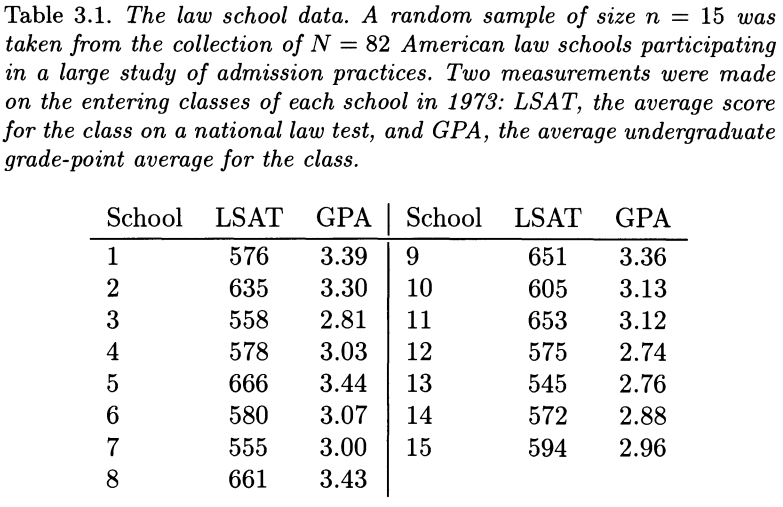
\includegraphics[width=\linewidth]{2/t21.png}
\newline

В таблице 3.1 показана случайная выборка размером $n = 15$, составленная из 82 американских юридических школ. Фактически показаны два измерения, проведенные для поступающих в 1973г. для каждого учебного заведения в выборке: LSAT, средний балл класса на экзамене по национальному праву, и GPA, средний балл бакалавриата, полученный студентами. В этом случае измерение $x_i$ на $u_i$, $i$-м члене выборки, представляет собой пару 
\begin{equation*}
    x_i=(LSAT_i, GPA_i)\quad i=1,2,\cdots,15
\end{equation*}
Наблюдаемые данные $x_1, x_2,\ldots, x_n$ представляют собой набор из 15 пар чисел, показанных в таблице 3.1. 

Этот пример является искусственным, потому что перепись данных $X_1, X_2,\cdots, X_82$ действительно была проведена. Другими словами, LSAT и GPA доступны для всей совокупности $N = 82$ школ. На Рисунке 3.1 показаны данные переписи и выборочные данные. В таблице 3.2 приведены все измерения $N$. 
\newline

\noindent
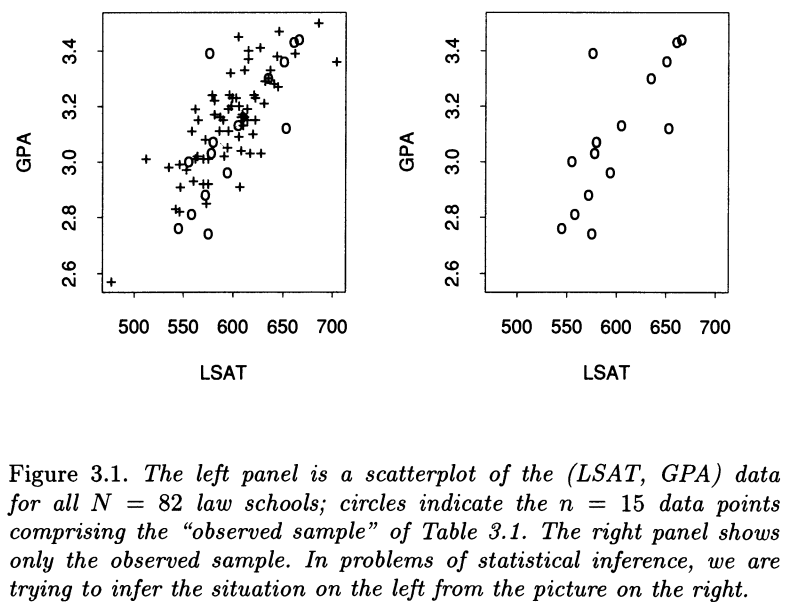
\includegraphics[width=\linewidth]{2/f31.png}
\newline

В реальной статистической задаче, такой как в таблице 3.1, мы увидим только выборочные данные, из которых мы попытаемся сделать вывод о свойствах совокупности. Например, рассмотрим 15 баллов LSAT в наблюдаемой выборке. Они имеют среднее значение $600.27$ с расчетной стандартной ошибкой $10.79$, основанной на данных в таблице 3.1 и формуле (2.2). Вероятность того, что истинное среднее значение LSAT, среднее для всей генеральной совокупности, из которой были взяты наблюдаемые данные, составляет около 68\%, находится в интервале $600.27 \pm 10.79$. 

Мы можем проверить этот результат, поскольку имеем дело с искусственным примером, для которого известны полные данные о населении. Среднее значение всех 82 значений LSAT составляет $597.55$, оно лежит в пределах прогнозируемого доверительного интервала $600.27 \pm 10.79$. 
\newline

\noindent
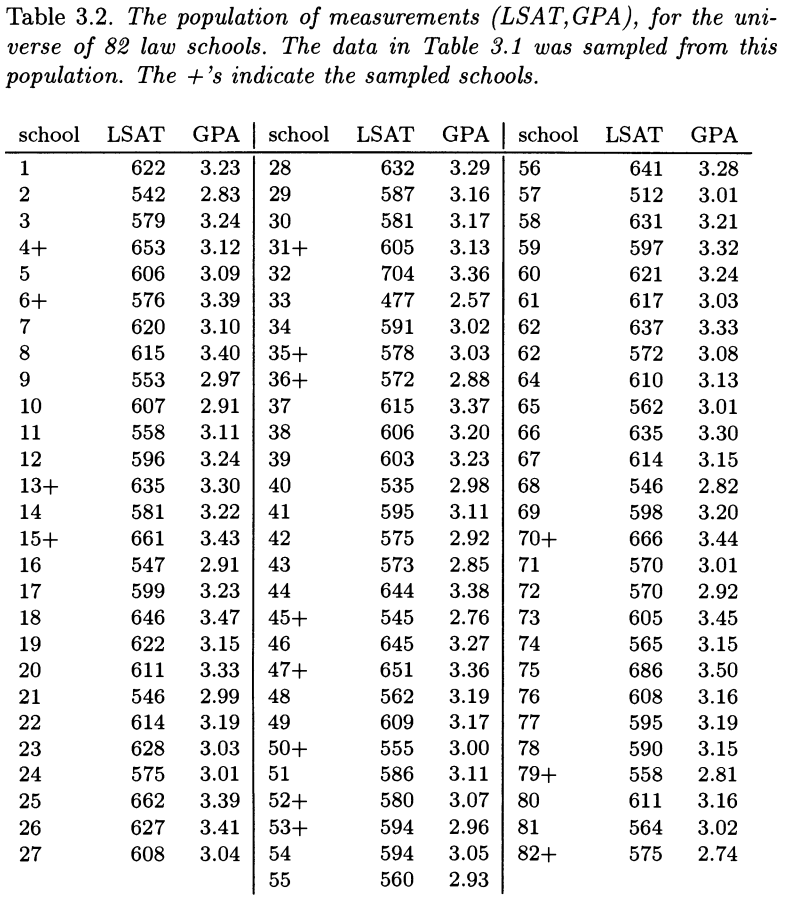
\includegraphics[width=\linewidth]{2/t32.png}
\newline